\documentclass{article}

\usepackage[a4paper, margin=2.7cm]{geometry}

\usepackage{biblatex}
\addbibresource{refs.bib}
\usepackage{graphicx}
\usepackage{microtype}
\usepackage{caption}
\usepackage{subcaption}
\usepackage{amsmath}
\usepackage{amssymb}
\DeclareMathOperator*{\argmax}{arg\,max}
\DeclareMathOperator*{\argmin}{arg\,min}
\DeclareMathOperator{\bel}{Bel}
\DeclareMathOperator{\expected}{E}

\usepackage{tikz}
\usetikzlibrary{arrows,shapes,positioning}


\begin{document}
\section{Abstract}
\section{Introduction}
What to observe is a choice that almost all living beings make constantly. Most creatures
have evolved significant flexibility in sensory apparatus which brings with it a great 
degree of freedom. Alongside this has developed an innate ability to effortlessly and
subconsciously decide how best to focus these resources. Reproducing this choice would 
be convenient in a number of situations from focusing computational effort on a small 
window of data, choosing a test or sensor to devote resources to or simply swivelling
a robotic head. In this {\textsc{writing}} we present a simple scenario fabricated
to compare several approaches to solving this general problem. 

\section{Related Work}
There is a significant body of work addressing related problems, but very little that 
moves beyond relatively \textit{ad-hoc} approaches tailored for specific goals or 
environments. We are looking at something related to Bacjsy's definition of Active 
Sensing, although hoping to sidestep the foundation in image processing.
\autocite{bajcsy1988active}

Following on from Bajcsy there is a large body of work regarding autonomous robotic 
heads, or at least mobile cameras. This kind of a system seems ideal, as it provides 
clear choices to shape the stream of incoming data. Despite this very little work
addresses the question of where to look in an abstract way, instead tending to code in 
desired behaviours by hand. Often this results in fixating on features particularly for 
simultaneous localisation and mapping \autocite{davison2002simultaneous, davison20013d}

A concept that seems related is the idea of salience in the context of image processing
and neuroscience.
The idea is to reproduce the eye movements of primates as a metric for which parts of
a scene are `interesting' in some way. Often a neuronal model can be applied after 
various steps of processing the input image. \autocite{itti1998salience} 
These kinds of models do seem to produce results similar to that of humans 
\autocite{parkhurst2002modeling} but the usefulness of these approaches appears to 
rest on the assumption that humans make good choices.

Something that arises from the salience literature is a split between `bottom up' and 
`top down' salience. The bottom-up components are the raw features which stand out
from the rest while the top down component is how the attention paid to these features 
is modulated by specific goals. \autocite{wolfe1994guided}

\section{Experimental Setup}
The goal of the experiments was to construct a simulation which captured some of the more
general issues. For simplicity everything was chosen to be discrete. It was necessary to
have a situation where the choice different choices of observation could lead to 
significantly different observations. The resulting scenario is localisation of an
autonomous agent on a known map. The world is small enough that beliefs can be handled
directly, which removes the need for approximation techniques.

The world state is simply the agents' two dimensional coordinates on an \(n \times n\)
grid, giving
\(n^2\) possible states. Each cell is either black or white with a single green
cell acting as the target, which the agents attempt to reach. The agents are free to 
move over any square -- the colour only affects the observations. 

At each time step agents are able to make a single observation of one of the adjacent
squares in either of the four cardinal directions: north, south east or west. These 
correspond to up, down, right or left respectively. Observations are drawn from the 
set of possible observations \(Y\) which simply contains representatives for black, 
white and green. There is some probability \(\rho_y\) (a parameter of the
simulation) that the correct observation will be made, with the two possible incorrect
observations having a corresponding \(\frac{(1-\rho_y)}{2}\) chance of being returned.
If the agent attempts to look off the edge of the board, it is treated as looking at a 
black cell.

After this the agents choose an action which manipulates the state, again one of the 
four cardinal directions. The result of this action is always to move the agent in the 
specified direction, except when they are attempting to move off the board in which case 
they simply remain in place. A summary of the steps that occur every time-step is 
given in figure \ref{fig:timestep}

\begin{figure}
\centering
\sffamily

\begin{enumerate}
	\item {Select sensor action \(a\) from set \(A\)}
	\item {Submit \(a\) to world, receive observation \(y \in Y\)}
	\item {Update beliefs according to sensor model \(P(y | a,x)\)}
	\item {Choose manipulatory action \(b \in B\)}
	\item {Advance state according to transition model \(P(x_{t+1} | b, x_t)\)}
	\item {Advance beliefs according to transition model \(P(x_{t+1} | b, x_t)\)}
\end{enumerate}

\caption{Sequence of events within each time-step of the simulation}
\label{fig:timestep}
\end{figure}

The desired behaviour was brought about by the predetermined value function 
\(U \colon X \to\mathbb{R}\) (\(X\) is the space of possible world states).
This function takes a set of coordinates \(x = (x_1, x_2)\) and returns the negative
Manhattan distance to the target --
\[
	U(x) = -(|x_1 - t_1| + |x_2 - t_2|)
\] where \((t_1, t_2)\) is the position of the target square. This is designed to 
simulate the sort of value function that might be learned by an agent in a world 
with a negative reward for every square except the target, which should encourage
locating the target as fast as possible.

\subsection{Maps}
Several different maps were used to test the different methods of choosing a sensor 
action. The first, seen in figure~\ref{fig:quarter} is divided into 4 quarters each
with a different pattern. The goal is always in the centre and the agents start in 
a randomly chosen corner. In order to reach the target, the agent must determine
which corner it is in. This map should then favour methods which focus on localising
quickly because as soon as the agent is localised sufficiently it can proceed to
take the shortest route to the centre.
\begin{figure}
\centering
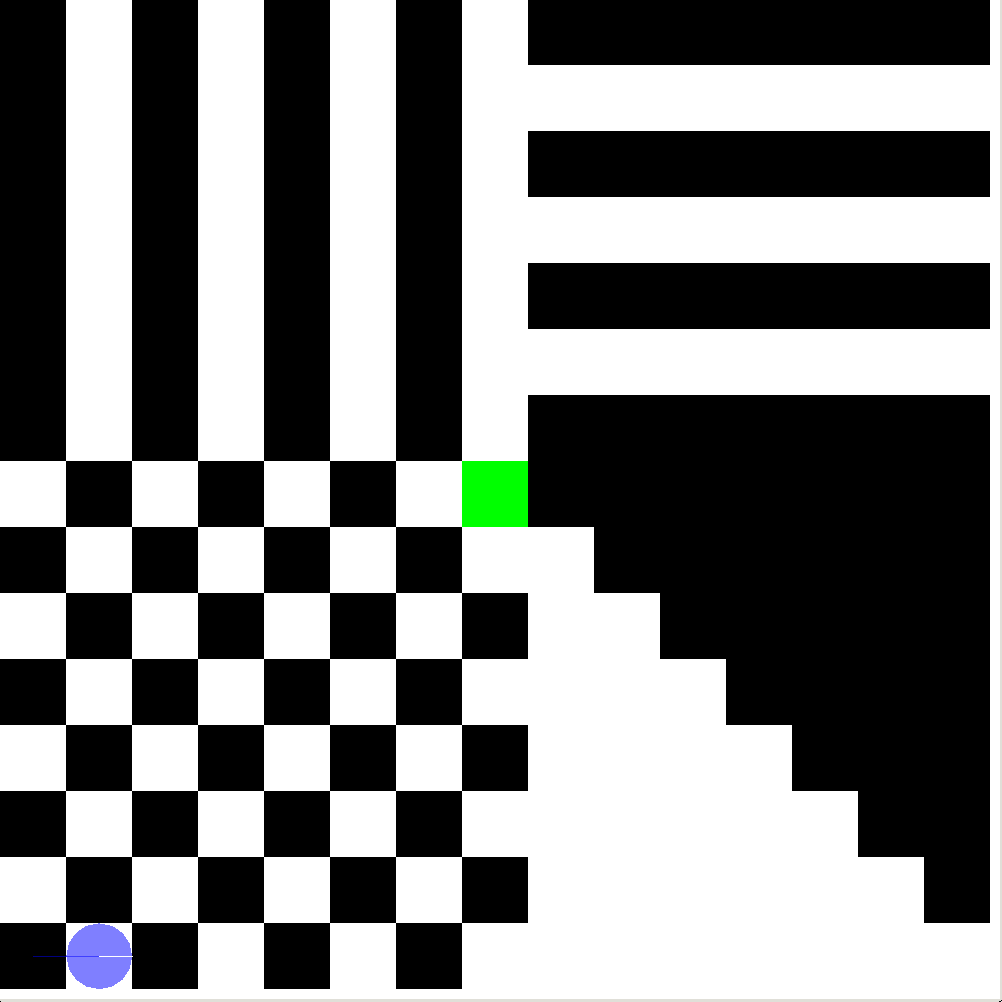
\includegraphics[width=\linewidth]{./figures/quartermap.png}
\caption{Map used for testing effect of changing sensor model. Agents start in 
a corner of the map, chosen randomly at the same trial. Trials were run concurrently 
with the group of agents all starting in the same corner. This map should favour those
that favour localisation as the best action is unclear until the agent is aware which 
corner it is in.}
\label{fig:quarter}
\end{figure}

To test in a more general setting with similar pressures, a large number of random maps
were also generated during testing. This was done by looping through every possible
square and deciding with a certain probability whether it should be black or white.
 The target was placed
afterwards. Adjusting the balance of black and white squares was done by changing the 
probability, which trades of the usefulness of a non-majority coloured square in 
localising with the chances of actually seeing one. 
Again the agents were placed at random corners
of a 15 by 15 map with a target in the middle, figure~\ref{fig:randommaps} shows 
some examples of these maps.

\begin{figure}
	\centering
	\begin{subfigure}[b]{0.2\linewidth}
		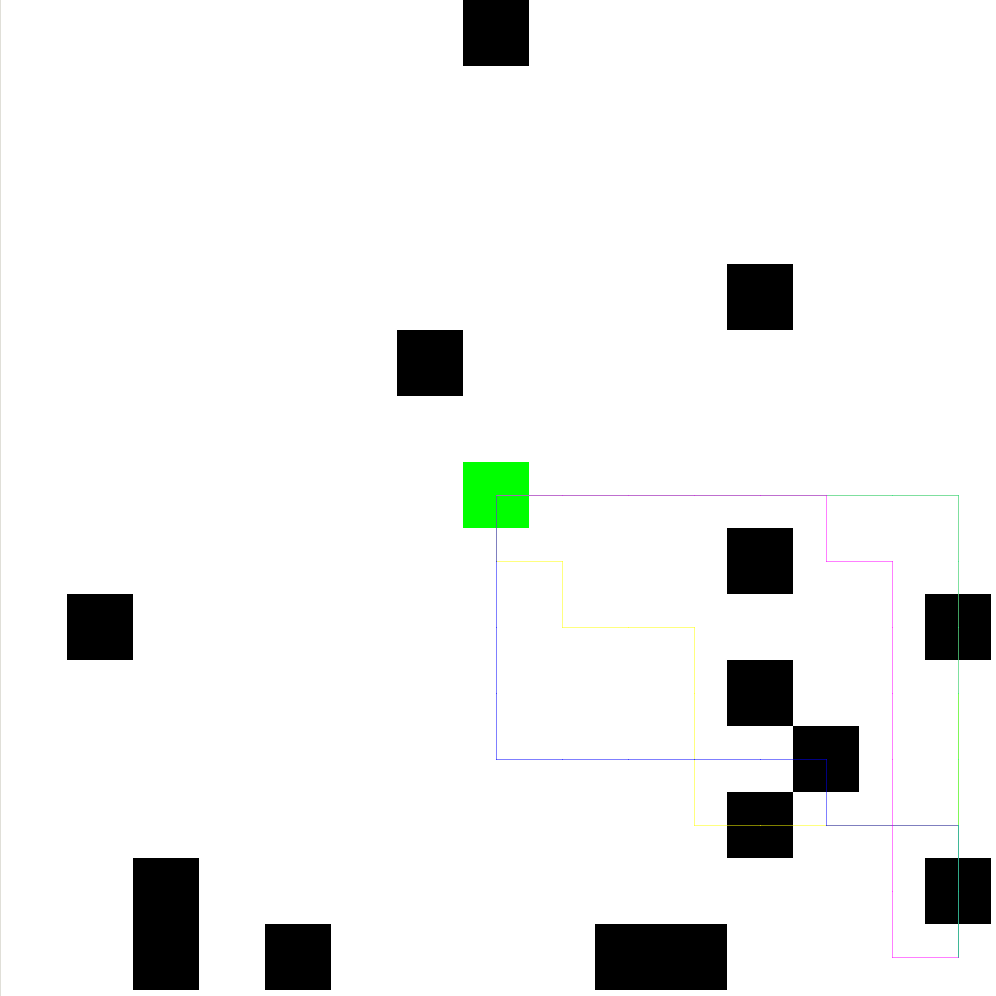
\includegraphics[width=1in]{./figures/randommap01}
		\caption{0.1}
	\end{subfigure}
	\begin{subfigure}[b]{0.2\linewidth}
		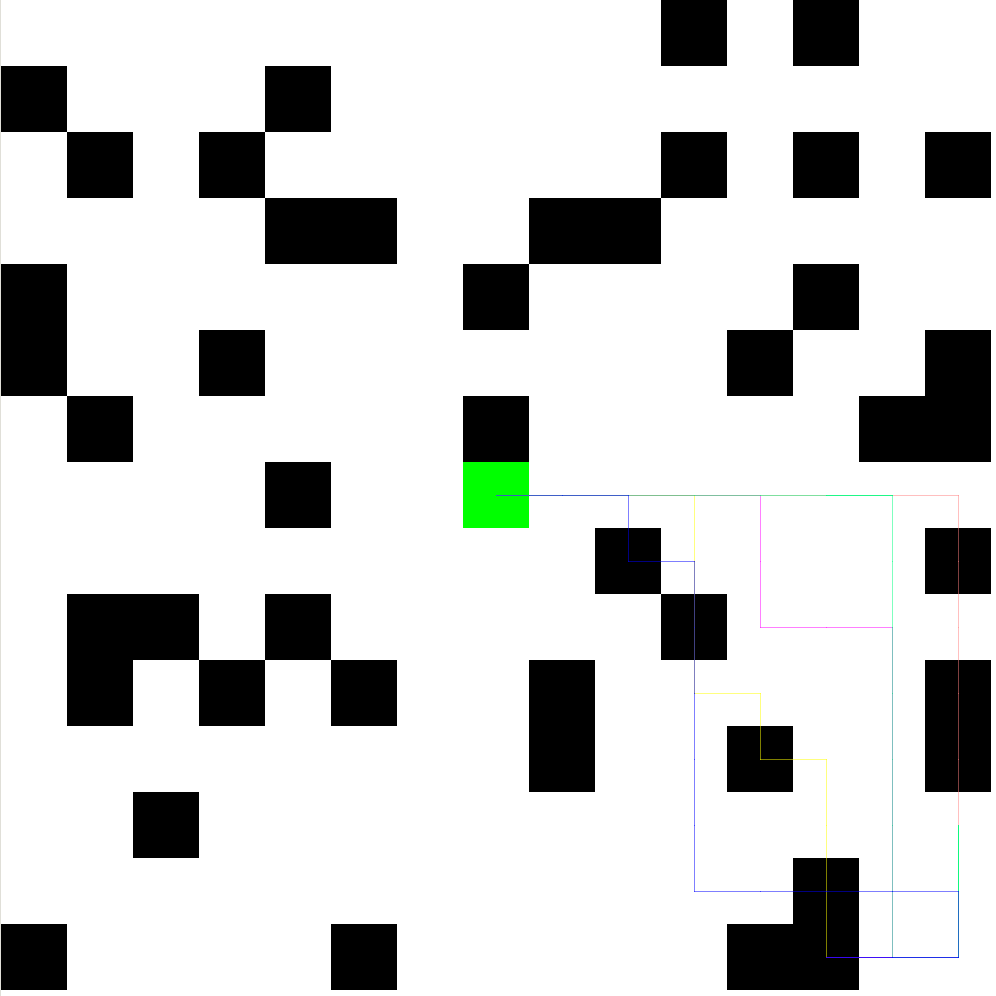
\includegraphics[width=1in]{./figures/randommap02}
		\caption{0.2}
	\end{subfigure}
	\begin{subfigure}[b]{0.2\linewidth}
		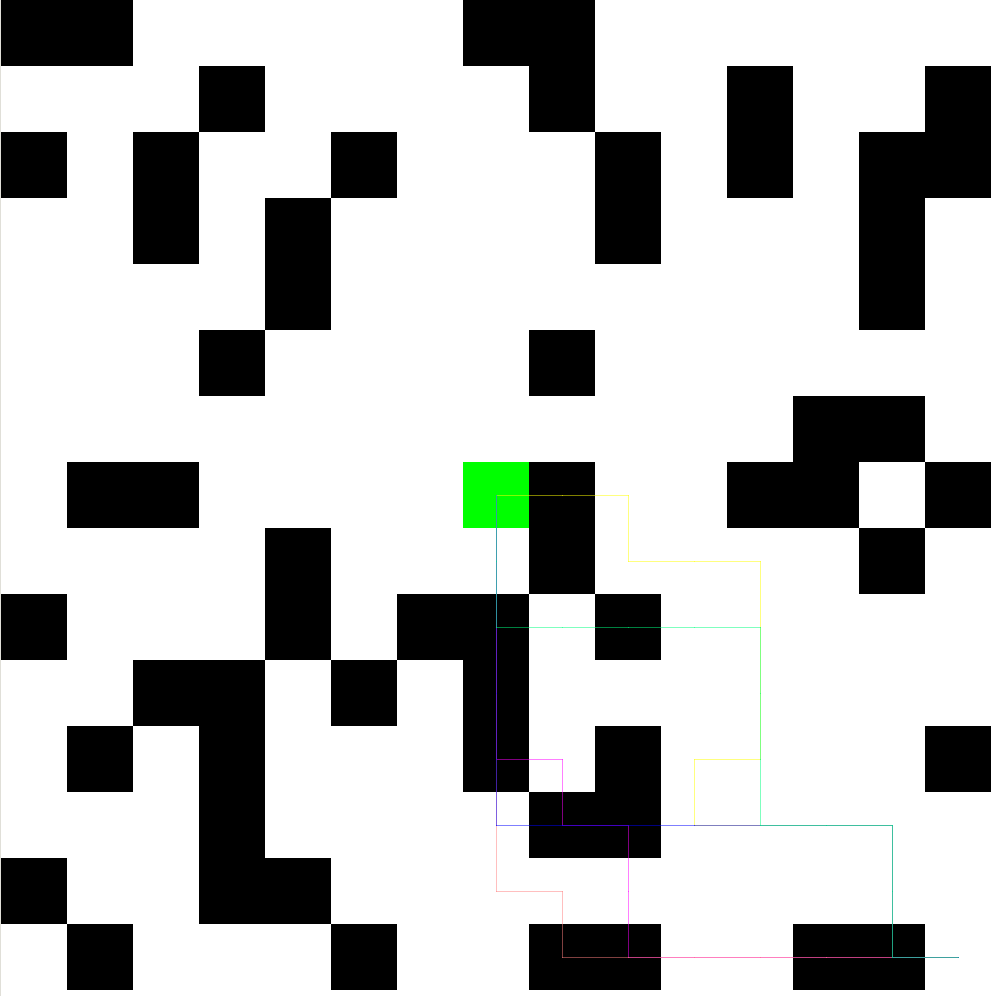
\includegraphics[width=1in]{./figures/randommap03}
		\caption{0.3}
	\end{subfigure}
	\begin{subfigure}[b]{0.2\linewidth}
		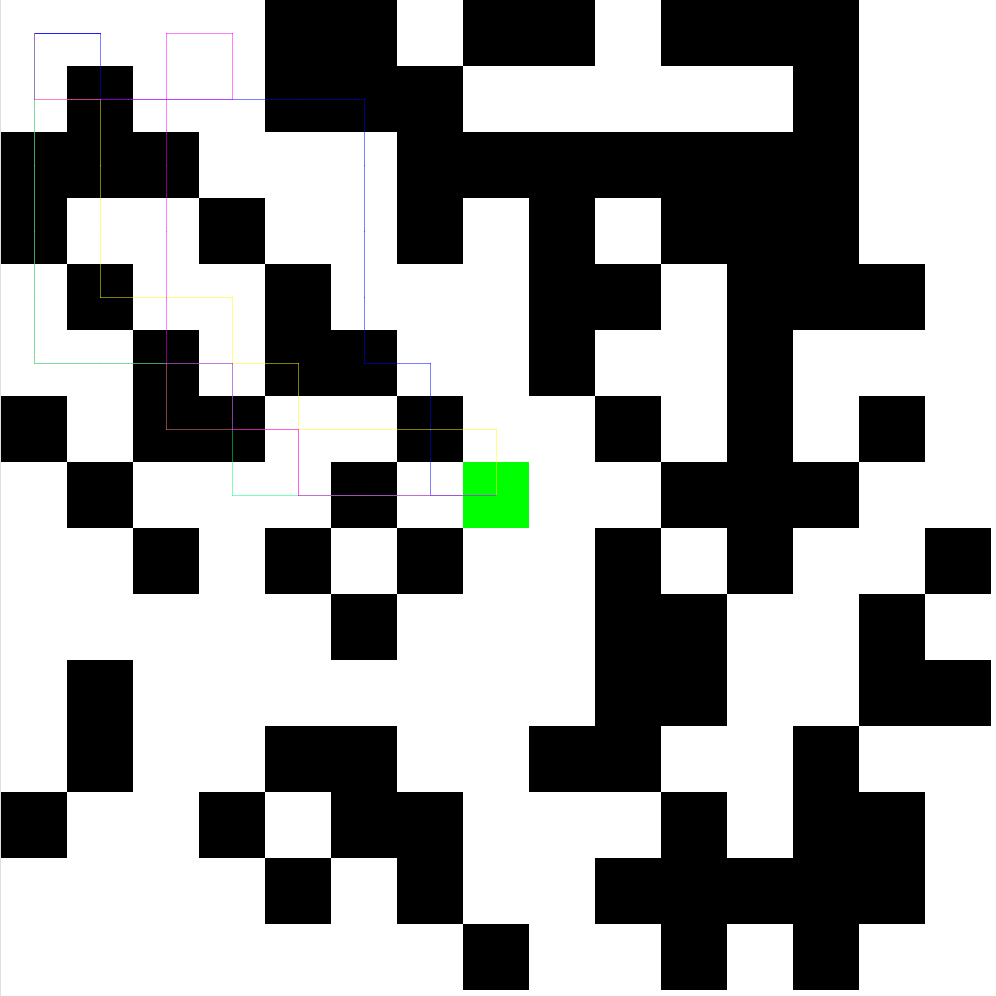
\includegraphics[width=1in]{./figures/randommap04}
		\caption{0.4}
	\end{subfigure}\\
	\begin{subfigure}[b]{0.2\linewidth}
		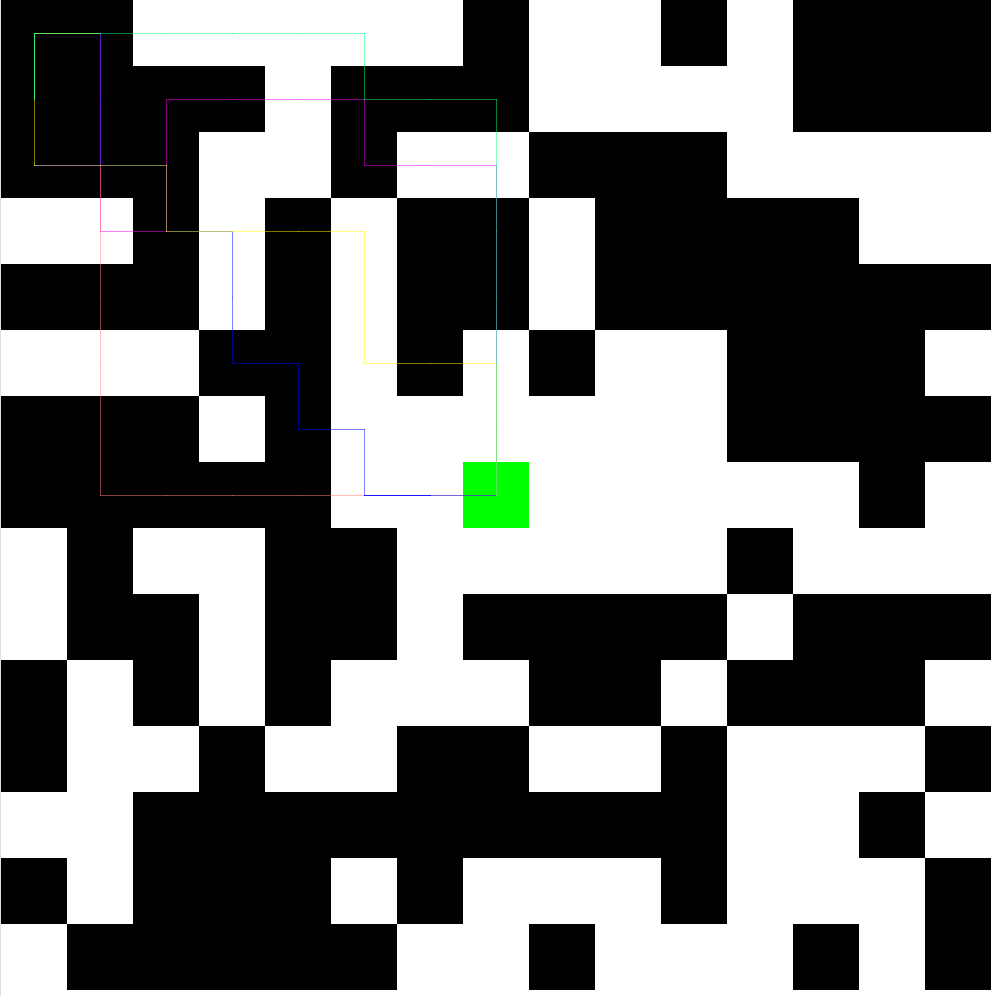
\includegraphics[width=1in]{./figures/randommap05}
		\caption{0.5}
	\end{subfigure}
	\begin{subfigure}[b]{0.2\linewidth}
		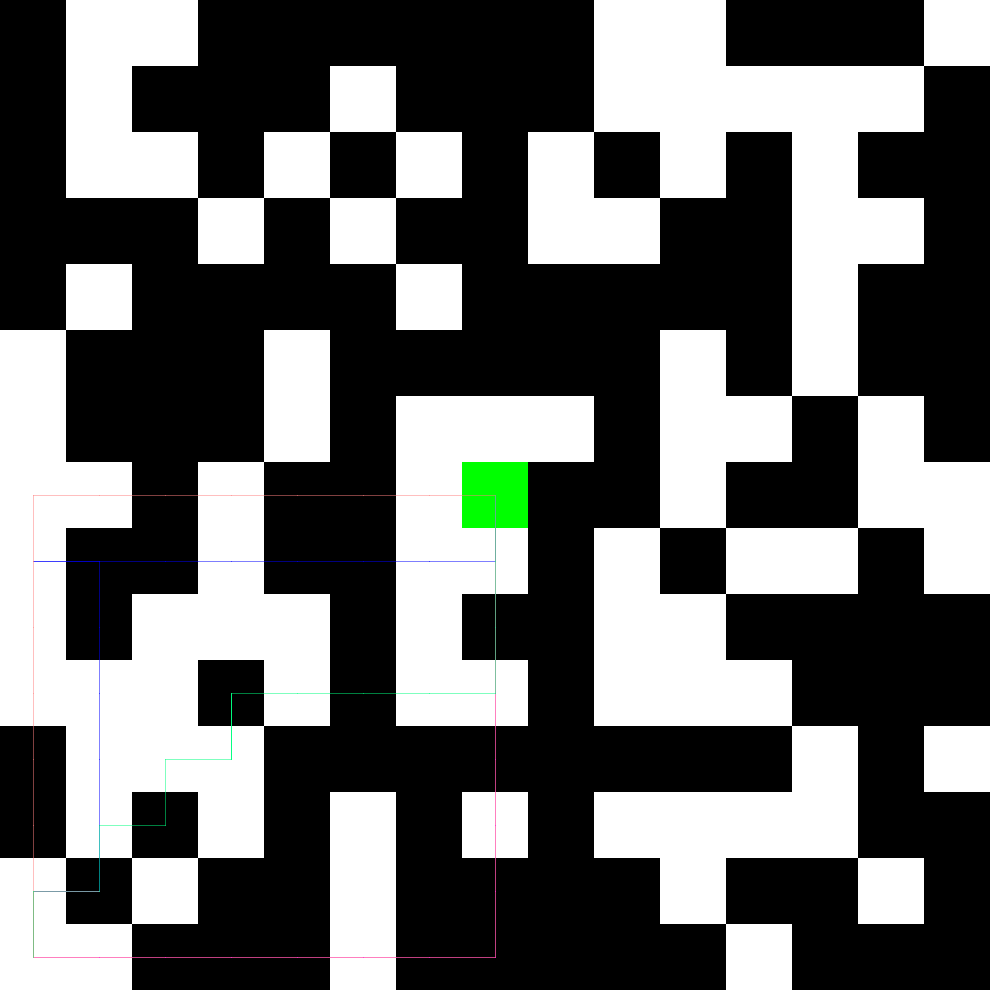
\includegraphics[width=1in]{./figures/randommap06}
		\caption{0.6}
	\end{subfigure}
	\begin{subfigure}[b]{0.2\linewidth}
		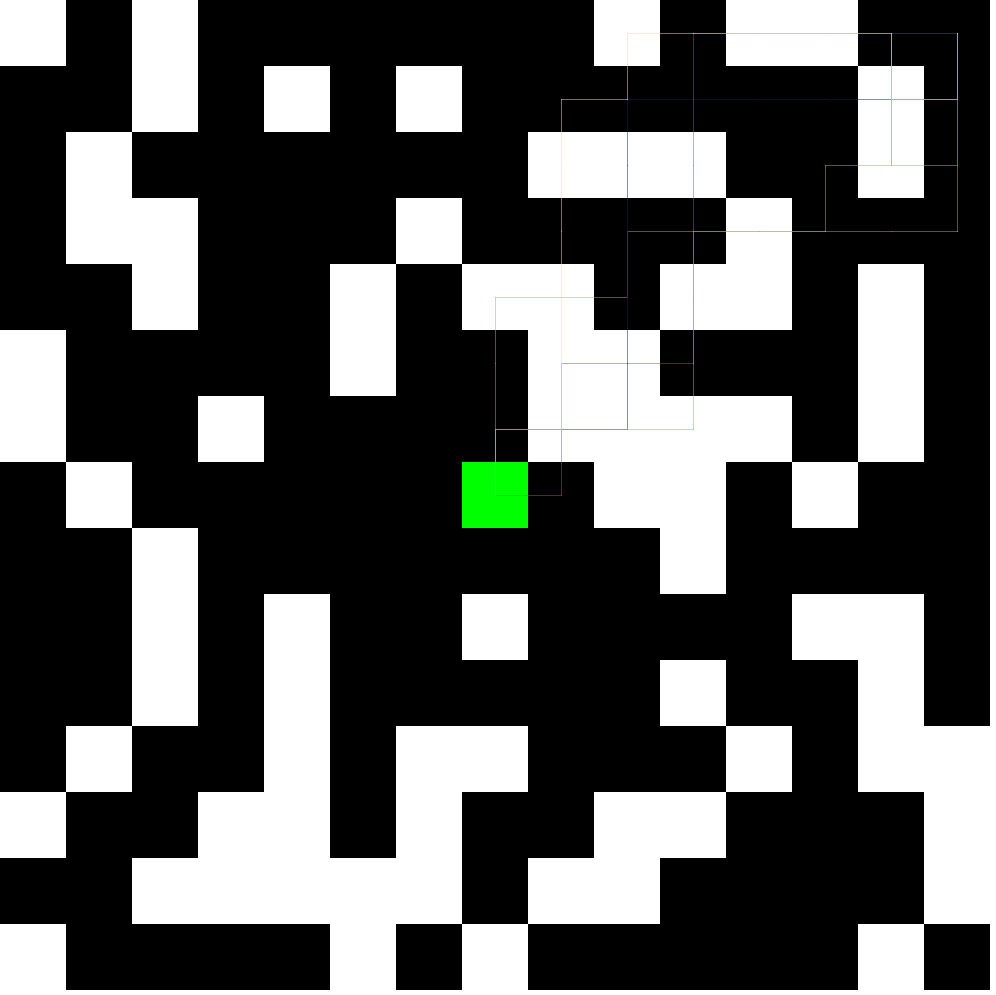
\includegraphics[width=1in]{./figures/randommap07}
		\caption{0.7}
	\end{subfigure}
	\begin{subfigure}[b]{0.2\linewidth}
		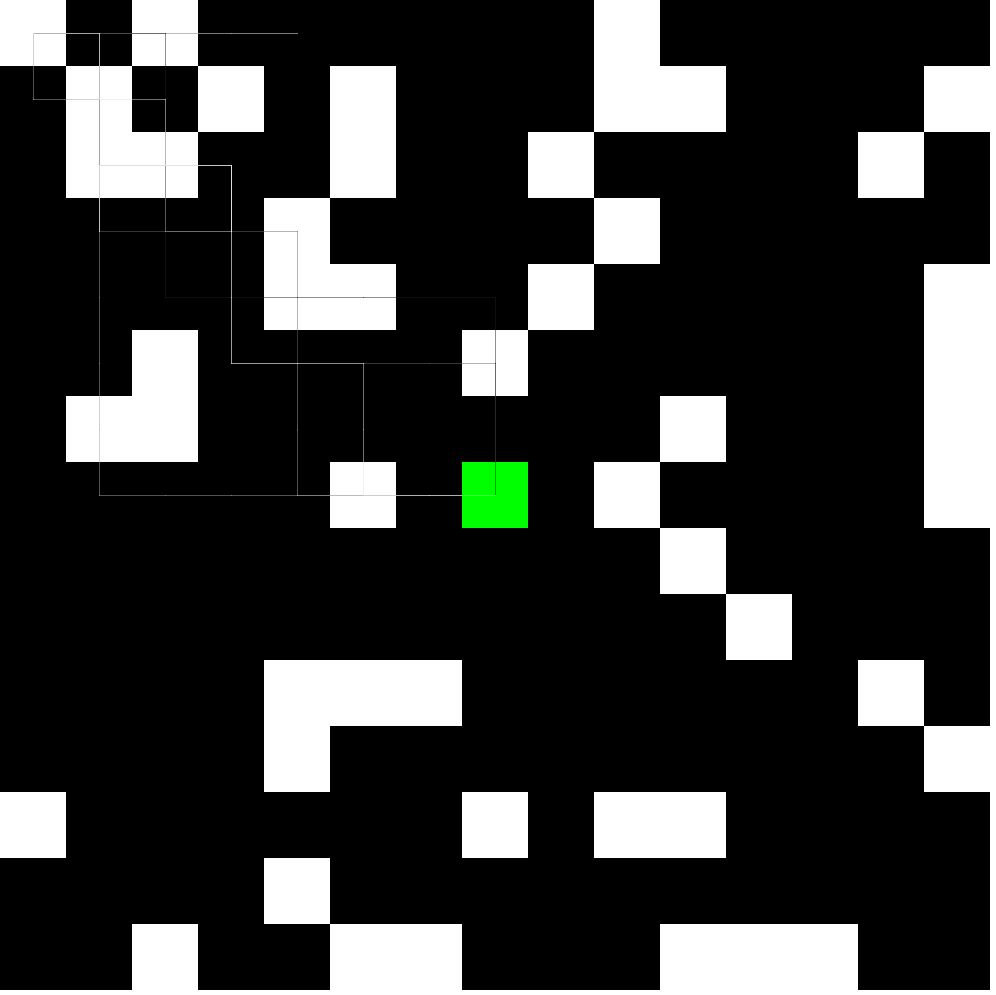
\includegraphics[width=1in]{./figures/randommap08}
		\caption{0.8}
	\end{subfigure}\\
	\begin{subfigure}[b]{0.2\linewidth}
		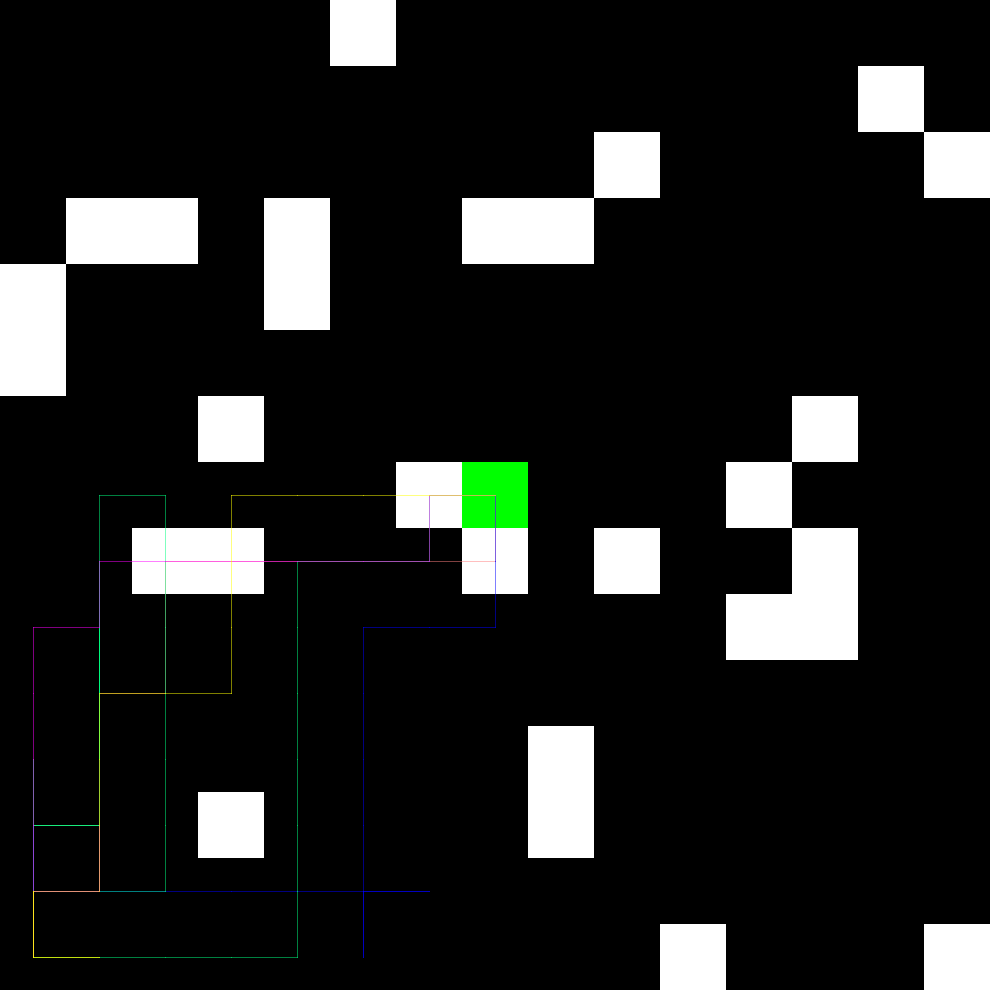
\includegraphics[width=1in]{./figures/randommap09}
		\caption{0.9}
	\end{subfigure}
	\caption{Examples of random maps with differing probabilities}
	\label{fig:randommaps}
\end{figure}



\section{Approaches}
The following details the different approaches for choosing a sensor action that were 
tested. All agents use precisely the same mechanism for choosing movement actions -- they
all maintain a belief distribution and choose greedily the action with the highest 
expected utility according to their beliefs. The difference comes in the actions used to 
shape those beliefs over time and this has a substantial impact on the performance of 
the agents.

\subsection{Basic Approach}
The simplest approach tested was to always look straight ahead. This can be seen as 
simulating a robot with a limited, fixed vision system -- the direction of the sensor is
always the same as the direction of the agents previous motion.

\subsection{Random}
A second simple approach was also tested alongside the more considered options: choosing
a random direction to look at every step. 

\subsection{Minimise Entropy}
This is the obvious approach if the goal is to localise the agent. In the case the goal of
the sensor action is to provide new beliefs with the lowest entropy possible. Thus for
each possible observation, we have to calculate the expected entropy over the resultant
belief states. This takes the form of a sum over all possible observations weighted by the
probability of receiving that observation. As the probability of an observation depends on
the state of the world, we have to sum over our current beliefs in order to determine the
observation probability. This yields: 
\[
	a^* \gets \argmin_{a \in A} \sum_{y \in {Y}} \sum_{x \in X} P(y|a,x) \bel(x) H(X')
\]
where \(H(X')\) is the entropy (using a base 2 logarithm) of the belief distribution
over \(X\) as it would be after having taken action \(a\) and received observation \(y\).


\subsection{Bayesian Surprise}
The motivation behind this approach is to maximise the amount of information gained by an
observation. This is achieved by maximising the relative entropy between the prior and the 
posterior beliefs after having made an observation.   
 \autocite{itti2005bayesian, baldi2010bits}
 
In order to choose the best sensor action we again compare the expected values across each 
possible action giving
\[
	a^* \gets \argmax_{a \in A} \sum_{y \in Y} \sum_{x \in X} P(y | a,x)\bel(x)K(\bel(X),\bel(X|a,y)).
\]
\(K(\bel(X), \bel(X|a,y))\) is the relative entropy, or Kullback-Leibler divergence, of 
the prior beliefs about \(X\) and where they would stand after an update, defined as
\[
	K(\bel(X), \bel(X | a,y) = \sum_{x \in X} \bel(x) \log \frac{\bel(x)}{\bel(x | a,y)}.
\] using a base \(e\) logarithm;

There are distinct similarities between the surprise approach and minimising entropy.
In particular the choice is governed entirely by the agents beliefs and should always
work to localise the agent quickly. Minimising entropy does this explicitly, but 
maximising surprise has similar behaviour in this world as the only actions that are going
to provide much surprise will be those with a reasonable chance of spotting a landmark
and thus helping the agent localise, reducing entropy of its beliefs.

\subsection{Goal-oriented}
\begin{figure}
\centering
	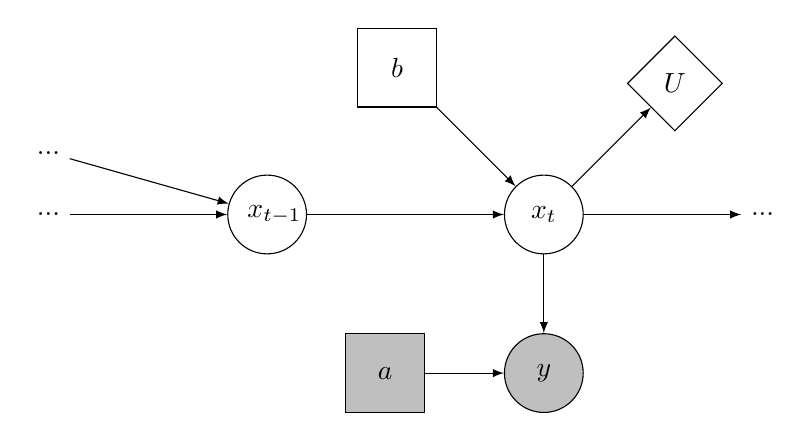
\begin{tikzpicture}
		[var/.style={draw,circle,text width=.5cm,minimum height=1cm, minimum width=1cm, align=center},							choice/.style={draw,rectangle,text width=.5cm, minimum height=1cm, minimum width=1cm, align=center},					reward/.style={draw,diamond,text width=.5cm,minimum height=1cm, minimum width=1cm, align=center}]
		
			\node[var](x) {\(x_t\)};
			\node[var, left =2.5cm of x](xold){\(x_{t-1}\)};
			\node[var, below=of x, fill=lightgray](y) {\(y\)};
			\node[choice, left=of y, fill=lightgray](a) {\(a\)};
			\node[choice, above left=of x](b) {\(b\)};
			\node[reward, above right=of x](g) {\(U\)};
			\node[left=2cm of xold](past){...};
			\node[right=2cm of x](future){...};
			\node[above=.5cm of past](pastb){...};
			
			\path
			(xold) edge[-latex] (x)
			(x) edge[-latex] (y)
			(a) edge[-latex] (y)
			(b) edge[-latex] (x)
			(x) edge[-latex] (g)
			(past) edge[-latex] (xold)
			(x) edge[-latex](future)
			(pastb) edge[-latex] (xold);

	\end{tikzpicture}
\caption{A model for the decision making process. Square nodes are choices while the 
diamond node is the reward, dependent on the state of the world. First \(a\) is chosen,
then \(y\) is observed then \(b\) is chosen then a reward is gathered and then the state
\(x\) advances, dependent on \(b\) and the current state of \(x\).}
\label{fig:ddn}
\end{figure}

This technique extends the approach used to choose the best movement action into
the realm of the sensor action. In order to derive this, it helps to look at 
figure~\ref{fig:ddn} which shows a graphical model of the process. The goal of the 
sensor action is then to maximise the reward obtained by the next choice. Thus we want
to choose \(a^*\) such that it maximises the expected utility of the next action:
\[
	a^* \gets \argmax_{a \in A} \expected_y \left[ U_{b^* | a,y}\right]
\]
\(U_{b* | a,y}\) is the utility of behaving optimally (taking action \(b^*\)) after
having taken sensor action \(a\) and receving observation \(y\). With discrete
observations, as we have here, the expected value is calculated as 
\(
	\expected_y \left[ U_{b^* | a,y}\right] = \sum_{y \in Y} \bel(y | a) U_{b^* | a,y}.
\)
To determine \(\bel(y | a)\) we have to look at the sensor model and our beliefs in the
state of the world: \(\bel(y | a) = \sum_{x_t \in X}  P(y | a,x_t)\bel(x_t).\) 

The utility of some action \(b\) given a sensor action \(a\) and an observation \(y\),
denoted \(U_{b | a,y}\), is the expected value (across beliefs in the world state) of 
the reward gathered after having taken action \(b\). This then depends on the beliefs
in the world state, the state transition model and the reward/value function \(U(x)\).
Specifically, the calculation is given as:
\[
	U_{b | a,t} = \sum_{x_t \in X} \sum_{x_{t+1} \in X} \bel(x_t | a,y)P(x_{t+1}|x_t,b)U(x_{t+1}).
\] The earlier equation calls for \(b^*\), the optimal choice of \(b\). It is optimal to 
choose the value which maximises the above quantity, hence we have a final expression
for the choice of sensor action
\[
	a^* \gets \argmax_{a \in A} \sum_{y \in Y} \sum_{x \in X} P(y | a,x)\bel(x) \max_{b \in B} \sum_{x_t \in X}\sum_{x_{t+1} \in X} \bel(x_t | a,y)P(x_{t+1}|x_t,b)U(x_{t+1}).
\]

This is a computationally complex sum to calculate, especially in worlds with a 
large number of possible states. Fortunately some savings can be made -- during each 
time step\(b^*\) is  dependent solely on the sensor action \(a\) and the observation
 \(y\). As both are discrete we can precompute a table containing \(b^*\) and 
 \(U_{b^* | a,y}\) for each \((a,y)\). This brings the complexity of the calculation
 more in line with the surprise approach.\footnote{Without precomputation, this approach
 is in \(\Theta(aybx^3)\) where \(a,y,b,x\) are the number of sensor actions, 
 observations, manipulatory actions and world states respectively. Precomputing
 pulls it into \(\Theta(aybx^2)\), which is a potentially significant gain in a complex
 world. By contrast calculating the surprise is in \(\Theta(ayx^2)\) as it is an argmax
 over \(A\) of a sum over \(Y\) of a sum over \(X\) of the KL divergence over \(X\) which
 is another sum over \(X\). Minimising entropy is in precisely the same class of 
 complexity as the only difference is taking the logarithm of the probability rather
 than the logarithm of a ratio of probabilities.}

\section{Results}

\begin{figure}
	\centering
	\begin{subfigure}[b]{\textwidth}
		% GNUPLOT: LaTeX picture with Postscript
\begingroup
  \makeatletter
  \providecommand\color[2][]{%
    \GenericError{(gnuplot) \space\space\space\@spaces}{%
      Package color not loaded in conjunction with
      terminal option `colourtext'%
    }{See the gnuplot documentation for explanation.%
    }{Either use 'blacktext' in gnuplot or load the package
      color.sty in LaTeX.}%
    \renewcommand\color[2][]{}%
  }%
  \providecommand\includegraphics[2][]{%
    \GenericError{(gnuplot) \space\space\space\@spaces}{%
      Package graphicx or graphics not loaded%
    }{See the gnuplot documentation for explanation.%
    }{The gnuplot epslatex terminal needs graphicx.sty or graphics.sty.}%
    \renewcommand\includegraphics[2][]{}%
  }%
  \providecommand\rotatebox[2]{#2}%
  \@ifundefined{ifGPcolor}{%
    \newif\ifGPcolor
    \GPcolortrue
  }{}%
  \@ifundefined{ifGPblacktext}{%
    \newif\ifGPblacktext
    \GPblacktexttrue
  }{}%
  % define a \g@addto@macro without @ in the name:
  \let\gplgaddtomacro\g@addto@macro
  % define empty templates for all commands taking text:
  \gdef\gplbacktext{}%
  \gdef\gplfronttext{}%
  \makeatother
  \ifGPblacktext
    % no textcolor at all
    \def\colorrgb#1{}%
    \def\colorgray#1{}%
  \else
    % gray or color?
    \ifGPcolor
      \def\colorrgb#1{\color[rgb]{#1}}%
      \def\colorgray#1{\color[gray]{#1}}%
      \expandafter\def\csname LTw\endcsname{\color{white}}%
      \expandafter\def\csname LTb\endcsname{\color{black}}%
      \expandafter\def\csname LTa\endcsname{\color{black}}%
      \expandafter\def\csname LT0\endcsname{\color[rgb]{1,0,0}}%
      \expandafter\def\csname LT1\endcsname{\color[rgb]{0,1,0}}%
      \expandafter\def\csname LT2\endcsname{\color[rgb]{0,0,1}}%
      \expandafter\def\csname LT3\endcsname{\color[rgb]{1,0,1}}%
      \expandafter\def\csname LT4\endcsname{\color[rgb]{0,1,1}}%
      \expandafter\def\csname LT5\endcsname{\color[rgb]{1,1,0}}%
      \expandafter\def\csname LT6\endcsname{\color[rgb]{0,0,0}}%
      \expandafter\def\csname LT7\endcsname{\color[rgb]{1,0.3,0}}%
      \expandafter\def\csname LT8\endcsname{\color[rgb]{0.5,0.5,0.5}}%
    \else
      % gray
      \def\colorrgb#1{\color{black}}%
      \def\colorgray#1{\color[gray]{#1}}%
      \expandafter\def\csname LTw\endcsname{\color{white}}%
      \expandafter\def\csname LTb\endcsname{\color{black}}%
      \expandafter\def\csname LTa\endcsname{\color{black}}%
      \expandafter\def\csname LT0\endcsname{\color{black}}%
      \expandafter\def\csname LT1\endcsname{\color{black}}%
      \expandafter\def\csname LT2\endcsname{\color{black}}%
      \expandafter\def\csname LT3\endcsname{\color{black}}%
      \expandafter\def\csname LT4\endcsname{\color{black}}%
      \expandafter\def\csname LT5\endcsname{\color{black}}%
      \expandafter\def\csname LT6\endcsname{\color{black}}%
      \expandafter\def\csname LT7\endcsname{\color{black}}%
      \expandafter\def\csname LT8\endcsname{\color{black}}%
    \fi
  \fi
  \setlength{\unitlength}{0.0500bp}%
  \begin{picture}(7200.00,5040.00)%
    \gplgaddtomacro\gplbacktext{%
      \csname LTb\endcsname%
      \put(726,440){\makebox(0,0)[r]{\strut{} 0}}%
      \put(726,1307){\makebox(0,0)[r]{\strut{} 50}}%
      \put(726,2174){\makebox(0,0)[r]{\strut{} 100}}%
      \put(726,3041){\makebox(0,0)[r]{\strut{} 150}}%
      \put(726,3908){\makebox(0,0)[r]{\strut{} 200}}%
      \put(726,4775){\makebox(0,0)[r]{\strut{} 250}}%
      \put(858,220){\makebox(0,0){\strut{} 0}}%
      \put(2047,220){\makebox(0,0){\strut{} 0.2}}%
      \put(3236,220){\makebox(0,0){\strut{} 0.4}}%
      \put(4425,220){\makebox(0,0){\strut{} 0.6}}%
      \put(5614,220){\makebox(0,0){\strut{} 0.8}}%
      \put(6803,220){\makebox(0,0){\strut{} 1}}%
    }%
    \gplgaddtomacro\gplfronttext{%
      \csname LTb\endcsname%
      \put(5816,4602){\makebox(0,0)[r]{\strut{}Random}}%
      \csname LTb\endcsname%
      \put(5816,4382){\makebox(0,0)[r]{\strut{}Surprise}}%
      \csname LTb\endcsname%
      \put(5816,4162){\makebox(0,0)[r]{\strut{}Entropy}}%
      \csname LTb\endcsname%
      \put(5816,3942){\makebox(0,0)[r]{\strut{}Optimal}}%
      \csname LTb\endcsname%
      \put(5816,3722){\makebox(0,0)[r]{\strut{}Straight Ahead}}%
    }%
    \gplbacktext
    \put(0,0){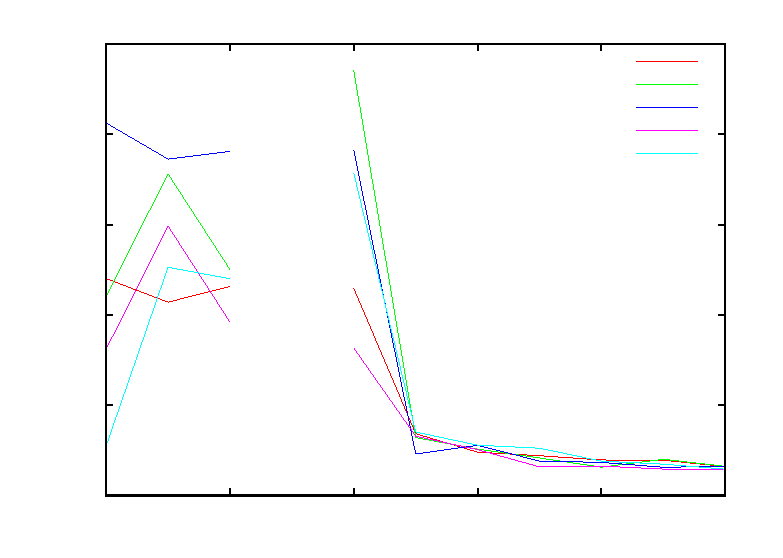
\includegraphics{./plots/obsprob}}%
    \gplfronttext
  \end{picture}%
\endgroup

		\caption{Average path length against observation probability}
		\label{fig:obsplot}
	\end{subfigure}
	\begin{subfigure}[b]{\textwidth}
		% GNUPLOT: LaTeX picture with Postscript
\begingroup
  \makeatletter
  \providecommand\color[2][]{%
    \GenericError{(gnuplot) \space\space\space\@spaces}{%
      Package color not loaded in conjunction with
      terminal option `colourtext'%
    }{See the gnuplot documentation for explanation.%
    }{Either use 'blacktext' in gnuplot or load the package
      color.sty in LaTeX.}%
    \renewcommand\color[2][]{}%
  }%
  \providecommand\includegraphics[2][]{%
    \GenericError{(gnuplot) \space\space\space\@spaces}{%
      Package graphicx or graphics not loaded%
    }{See the gnuplot documentation for explanation.%
    }{The gnuplot epslatex terminal needs graphicx.sty or graphics.sty.}%
    \renewcommand\includegraphics[2][]{}%
  }%
  \providecommand\rotatebox[2]{#2}%
  \@ifundefined{ifGPcolor}{%
    \newif\ifGPcolor
    \GPcolortrue
  }{}%
  \@ifundefined{ifGPblacktext}{%
    \newif\ifGPblacktext
    \GPblacktexttrue
  }{}%
  % define a \g@addto@macro without @ in the name:
  \let\gplgaddtomacro\g@addto@macro
  % define empty templates for all commands taking text:
  \gdef\gplbacktext{}%
  \gdef\gplfronttext{}%
  \makeatother
  \ifGPblacktext
    % no textcolor at all
    \def\colorrgb#1{}%
    \def\colorgray#1{}%
  \else
    % gray or color?
    \ifGPcolor
      \def\colorrgb#1{\color[rgb]{#1}}%
      \def\colorgray#1{\color[gray]{#1}}%
      \expandafter\def\csname LTw\endcsname{\color{white}}%
      \expandafter\def\csname LTb\endcsname{\color{black}}%
      \expandafter\def\csname LTa\endcsname{\color{black}}%
      \expandafter\def\csname LT0\endcsname{\color[rgb]{1,0,0}}%
      \expandafter\def\csname LT1\endcsname{\color[rgb]{0,1,0}}%
      \expandafter\def\csname LT2\endcsname{\color[rgb]{0,0,1}}%
      \expandafter\def\csname LT3\endcsname{\color[rgb]{1,0,1}}%
      \expandafter\def\csname LT4\endcsname{\color[rgb]{0,1,1}}%
      \expandafter\def\csname LT5\endcsname{\color[rgb]{1,1,0}}%
      \expandafter\def\csname LT6\endcsname{\color[rgb]{0,0,0}}%
      \expandafter\def\csname LT7\endcsname{\color[rgb]{1,0.3,0}}%
      \expandafter\def\csname LT8\endcsname{\color[rgb]{0.5,0.5,0.5}}%
    \else
      % gray
      \def\colorrgb#1{\color{black}}%
      \def\colorgray#1{\color[gray]{#1}}%
      \expandafter\def\csname LTw\endcsname{\color{white}}%
      \expandafter\def\csname LTb\endcsname{\color{black}}%
      \expandafter\def\csname LTa\endcsname{\color{black}}%
      \expandafter\def\csname LT0\endcsname{\color{black}}%
      \expandafter\def\csname LT1\endcsname{\color{black}}%
      \expandafter\def\csname LT2\endcsname{\color{black}}%
      \expandafter\def\csname LT3\endcsname{\color{black}}%
      \expandafter\def\csname LT4\endcsname{\color{black}}%
      \expandafter\def\csname LT5\endcsname{\color{black}}%
      \expandafter\def\csname LT6\endcsname{\color{black}}%
      \expandafter\def\csname LT7\endcsname{\color{black}}%
      \expandafter\def\csname LT8\endcsname{\color{black}}%
    \fi
  \fi
  \setlength{\unitlength}{0.0500bp}%
  \begin{picture}(7200.00,5040.00)%
    \gplgaddtomacro\gplbacktext{%
      \csname LTb\endcsname%
      \put(594,440){\makebox(0,0)[r]{\strut{} 10}}%
      \put(594,1163){\makebox(0,0)[r]{\strut{} 15}}%
      \put(594,1885){\makebox(0,0)[r]{\strut{} 20}}%
      \put(594,2608){\makebox(0,0)[r]{\strut{} 25}}%
      \put(594,3330){\makebox(0,0)[r]{\strut{} 30}}%
      \put(594,4053){\makebox(0,0)[r]{\strut{} 35}}%
      \put(594,4775){\makebox(0,0)[r]{\strut{} 40}}%
      \put(726,220){\makebox(0,0){\strut{} 0.5}}%
      \put(1941,220){\makebox(0,0){\strut{} 0.6}}%
      \put(3157,220){\makebox(0,0){\strut{} 0.7}}%
      \put(4372,220){\makebox(0,0){\strut{} 0.8}}%
      \put(5588,220){\makebox(0,0){\strut{} 0.9}}%
      \put(6803,220){\makebox(0,0){\strut{} 1}}%
    }%
    \gplgaddtomacro\gplfronttext{%
      \csname LTb\endcsname%
      \put(5816,4602){\makebox(0,0)[r]{\strut{}Random}}%
      \csname LTb\endcsname%
      \put(5816,4382){\makebox(0,0)[r]{\strut{}Surprise}}%
      \csname LTb\endcsname%
      \put(5816,4162){\makebox(0,0)[r]{\strut{}Entropy}}%
      \csname LTb\endcsname%
      \put(5816,3942){\makebox(0,0)[r]{\strut{}Optimal}}%
      \csname LTb\endcsname%
      \put(5816,3722){\makebox(0,0)[r]{\strut{}Straight Ahead}}%
    }%
    \gplbacktext
    \put(0,0){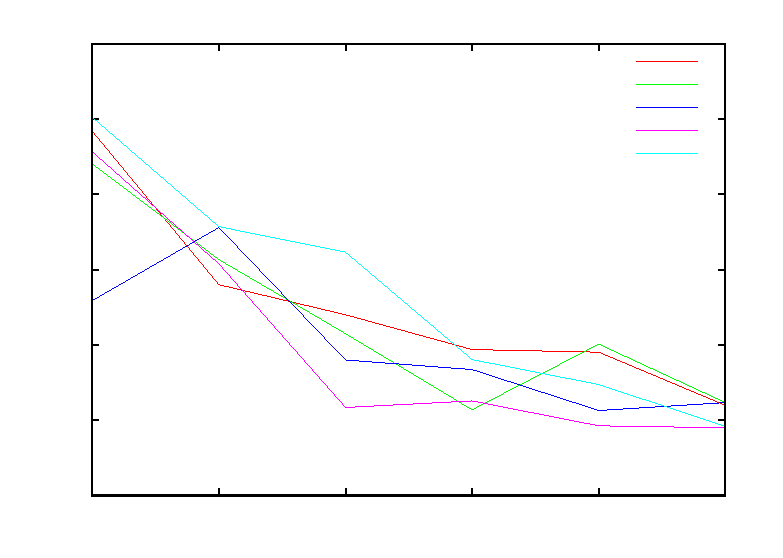
\includegraphics{./plots/obsplotmag}}%
    \gplfronttext
  \end{picture}%
\endgroup

		\caption{The same plot, focusing on probabilities 0.5 and greater}
		\label{fig:obsplotmag}
	\end{subfigure}
	\caption{Results of 15 by 15 quarter map, averages across 2500 trials.}
	\label{fig:obsres}
\end{figure}

The first set of trials were conducted on the map in figure~\ref{fig:quarter}. The 
average path length was measured across 2500 trials for ten different values of 
\(\rho_y\), the probability of a correct observation which were evenly spaced between
zero and one. Results can be seen in figure~\ref{fig:obsplot} for the 15 by 15 map, 
which has a shortest possible path of 14. As the uncertainty of the
observation increases, the simulation breaks down. When there is almost nothing to be
learned from the observations (\(\rho_y = 0.3\)) none of the approaches was able to 
complete a single trial within 300 steps. Up until \(\rho_y = 0.5\) the goal-driven
agent leads the pack. It is quite close but this approach seems to outperform several
others as the uncertainty around the observation starts to increase.

This might make sense. As the observations become less useful, it becomes much harder
for the agents to reduce the entropy of their beliefs or glean much information from 
the observation and as such the choices of the approaches based on these ideas is not 
much better than choosing randomly. The goal-oriented agent is not as worried about its
beliefs as a whole, it will favour choices which might let it believe the goal is 
imminently attainable. Intuitively this should lead to more sensible decision making
in situations where localisation is difficult and to better performance in circumstances
where precise localisation is not strictly necessary to achieve the goal.

Subsequent trials took place on randomised maps and were highly inconclusive, even 
when results were taken over 10000 trials (on a smaller map due to time constraints).
Figure~\ref{fig:smallrand} shows the average lengths plotted agains the probability
of an individula square in the map being black. The individual approaches are 
inseparable and incredibly noisy. There is a clear upwards trend as the likelihood
of very many white squares decreases. This is evident on the larger map as well in
figures \ref{fig:random80} and \ref{fig:random90}. This is to be expected given that 
any time an agent looks off the end of the map it is treated as looking at a black 
square. This is like having an implicit border of black squares, which means that when
the majority of the map is white, being in a corner is a very good position in which to 
localise. Conversely when most of the squares are black there is very little assistance 
anywhere, so we would expect the agents to perform worse, which they all appear to.


\begin{figure}
	% GNUPLOT: LaTeX picture with Postscript
\begingroup
  \makeatletter
  \providecommand\color[2][]{%
    \GenericError{(gnuplot) \space\space\space\@spaces}{%
      Package color not loaded in conjunction with
      terminal option `colourtext'%
    }{See the gnuplot documentation for explanation.%
    }{Either use 'blacktext' in gnuplot or load the package
      color.sty in LaTeX.}%
    \renewcommand\color[2][]{}%
  }%
  \providecommand\includegraphics[2][]{%
    \GenericError{(gnuplot) \space\space\space\@spaces}{%
      Package graphicx or graphics not loaded%
    }{See the gnuplot documentation for explanation.%
    }{The gnuplot epslatex terminal needs graphicx.sty or graphics.sty.}%
    \renewcommand\includegraphics[2][]{}%
  }%
  \providecommand\rotatebox[2]{#2}%
  \@ifundefined{ifGPcolor}{%
    \newif\ifGPcolor
    \GPcolortrue
  }{}%
  \@ifundefined{ifGPblacktext}{%
    \newif\ifGPblacktext
    \GPblacktexttrue
  }{}%
  % define a \g@addto@macro without @ in the name:
  \let\gplgaddtomacro\g@addto@macro
  % define empty templates for all commands taking text:
  \gdef\gplbacktext{}%
  \gdef\gplfronttext{}%
  \makeatother
  \ifGPblacktext
    % no textcolor at all
    \def\colorrgb#1{}%
    \def\colorgray#1{}%
  \else
    % gray or color?
    \ifGPcolor
      \def\colorrgb#1{\color[rgb]{#1}}%
      \def\colorgray#1{\color[gray]{#1}}%
      \expandafter\def\csname LTw\endcsname{\color{white}}%
      \expandafter\def\csname LTb\endcsname{\color{black}}%
      \expandafter\def\csname LTa\endcsname{\color{black}}%
      \expandafter\def\csname LT0\endcsname{\color[rgb]{1,0,0}}%
      \expandafter\def\csname LT1\endcsname{\color[rgb]{0,1,0}}%
      \expandafter\def\csname LT2\endcsname{\color[rgb]{0,0,1}}%
      \expandafter\def\csname LT3\endcsname{\color[rgb]{1,0,1}}%
      \expandafter\def\csname LT4\endcsname{\color[rgb]{0,1,1}}%
      \expandafter\def\csname LT5\endcsname{\color[rgb]{1,1,0}}%
      \expandafter\def\csname LT6\endcsname{\color[rgb]{0,0,0}}%
      \expandafter\def\csname LT7\endcsname{\color[rgb]{1,0.3,0}}%
      \expandafter\def\csname LT8\endcsname{\color[rgb]{0.5,0.5,0.5}}%
    \else
      % gray
      \def\colorrgb#1{\color{black}}%
      \def\colorgray#1{\color[gray]{#1}}%
      \expandafter\def\csname LTw\endcsname{\color{white}}%
      \expandafter\def\csname LTb\endcsname{\color{black}}%
      \expandafter\def\csname LTa\endcsname{\color{black}}%
      \expandafter\def\csname LT0\endcsname{\color{black}}%
      \expandafter\def\csname LT1\endcsname{\color{black}}%
      \expandafter\def\csname LT2\endcsname{\color{black}}%
      \expandafter\def\csname LT3\endcsname{\color{black}}%
      \expandafter\def\csname LT4\endcsname{\color{black}}%
      \expandafter\def\csname LT5\endcsname{\color{black}}%
      \expandafter\def\csname LT6\endcsname{\color{black}}%
      \expandafter\def\csname LT7\endcsname{\color{black}}%
      \expandafter\def\csname LT8\endcsname{\color{black}}%
    \fi
  \fi
  \setlength{\unitlength}{0.0500bp}%
  \begin{picture}(7200.00,5040.00)%
    \gplgaddtomacro\gplbacktext{%
      \csname LTb\endcsname%
      \put(594,440){\makebox(0,0)[r]{\strut{} 6}}%
      \put(594,1163){\makebox(0,0)[r]{\strut{} 8}}%
      \put(594,1885){\makebox(0,0)[r]{\strut{} 10}}%
      \put(594,2608){\makebox(0,0)[r]{\strut{} 12}}%
      \put(594,3330){\makebox(0,0)[r]{\strut{} 14}}%
      \put(594,4053){\makebox(0,0)[r]{\strut{} 16}}%
      \put(594,4775){\makebox(0,0)[r]{\strut{} 18}}%
      \put(726,220){\makebox(0,0){\strut{} 0.1}}%
      \put(1486,220){\makebox(0,0){\strut{} 0.2}}%
      \put(2245,220){\makebox(0,0){\strut{} 0.3}}%
      \put(3005,220){\makebox(0,0){\strut{} 0.4}}%
      \put(3765,220){\makebox(0,0){\strut{} 0.5}}%
      \put(4524,220){\makebox(0,0){\strut{} 0.6}}%
      \put(5284,220){\makebox(0,0){\strut{} 0.7}}%
      \put(6043,220){\makebox(0,0){\strut{} 0.8}}%
      \put(6803,220){\makebox(0,0){\strut{} 0.9}}%
    }%
    \gplgaddtomacro\gplfronttext{%
      \csname LTb\endcsname%
      \put(5816,4602){\makebox(0,0)[r]{\strut{}Random}}%
      \csname LTb\endcsname%
      \put(5816,4382){\makebox(0,0)[r]{\strut{}Surprise}}%
      \csname LTb\endcsname%
      \put(5816,4162){\makebox(0,0)[r]{\strut{}Entropy}}%
      \csname LTb\endcsname%
      \put(5816,3942){\makebox(0,0)[r]{\strut{}Optimal}}%
      \csname LTb\endcsname%
      \put(5816,3722){\makebox(0,0)[r]{\strut{}Straight Ahead}}%
    }%
    \gplbacktext
    \put(0,0){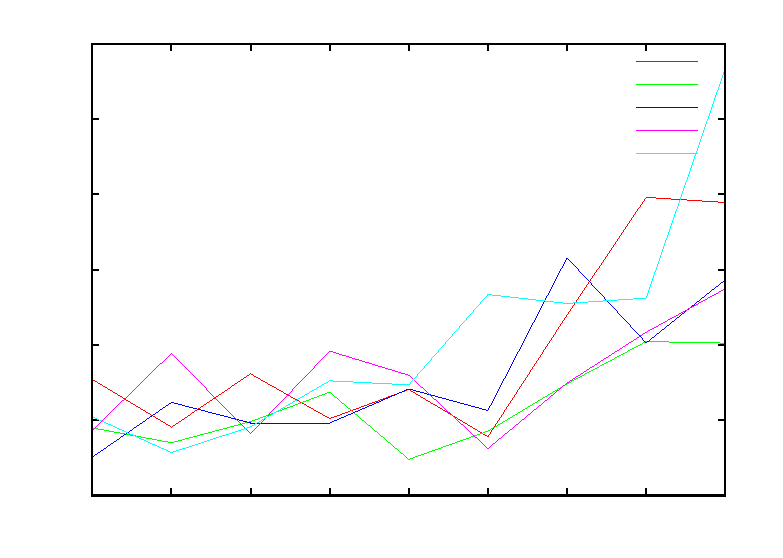
\includegraphics{./plots/randommapsmall}}%
    \gplfronttext
  \end{picture}%
\endgroup

	\caption{Average path length over 10000 trials on an 7 by 7 random map. Shortest 
	possible path was 6 steps}
	\label{fig:smallrand}
\end{figure}
\begin{figure}
	% GNUPLOT: LaTeX picture with Postscript
\begingroup
  \makeatletter
  \providecommand\color[2][]{%
    \GenericError{(gnuplot) \space\space\space\@spaces}{%
      Package color not loaded in conjunction with
      terminal option `colourtext'%
    }{See the gnuplot documentation for explanation.%
    }{Either use 'blacktext' in gnuplot or load the package
      color.sty in LaTeX.}%
    \renewcommand\color[2][]{}%
  }%
  \providecommand\includegraphics[2][]{%
    \GenericError{(gnuplot) \space\space\space\@spaces}{%
      Package graphicx or graphics not loaded%
    }{See the gnuplot documentation for explanation.%
    }{The gnuplot epslatex terminal needs graphicx.sty or graphics.sty.}%
    \renewcommand\includegraphics[2][]{}%
  }%
  \providecommand\rotatebox[2]{#2}%
  \@ifundefined{ifGPcolor}{%
    \newif\ifGPcolor
    \GPcolortrue
  }{}%
  \@ifundefined{ifGPblacktext}{%
    \newif\ifGPblacktext
    \GPblacktexttrue
  }{}%
  % define a \g@addto@macro without @ in the name:
  \let\gplgaddtomacro\g@addto@macro
  % define empty templates for all commands taking text:
  \gdef\gplbacktext{}%
  \gdef\gplfronttext{}%
  \makeatother
  \ifGPblacktext
    % no textcolor at all
    \def\colorrgb#1{}%
    \def\colorgray#1{}%
  \else
    % gray or color?
    \ifGPcolor
      \def\colorrgb#1{\color[rgb]{#1}}%
      \def\colorgray#1{\color[gray]{#1}}%
      \expandafter\def\csname LTw\endcsname{\color{white}}%
      \expandafter\def\csname LTb\endcsname{\color{black}}%
      \expandafter\def\csname LTa\endcsname{\color{black}}%
      \expandafter\def\csname LT0\endcsname{\color[rgb]{1,0,0}}%
      \expandafter\def\csname LT1\endcsname{\color[rgb]{0,1,0}}%
      \expandafter\def\csname LT2\endcsname{\color[rgb]{0,0,1}}%
      \expandafter\def\csname LT3\endcsname{\color[rgb]{1,0,1}}%
      \expandafter\def\csname LT4\endcsname{\color[rgb]{0,1,1}}%
      \expandafter\def\csname LT5\endcsname{\color[rgb]{1,1,0}}%
      \expandafter\def\csname LT6\endcsname{\color[rgb]{0,0,0}}%
      \expandafter\def\csname LT7\endcsname{\color[rgb]{1,0.3,0}}%
      \expandafter\def\csname LT8\endcsname{\color[rgb]{0.5,0.5,0.5}}%
    \else
      % gray
      \def\colorrgb#1{\color{black}}%
      \def\colorgray#1{\color[gray]{#1}}%
      \expandafter\def\csname LTw\endcsname{\color{white}}%
      \expandafter\def\csname LTb\endcsname{\color{black}}%
      \expandafter\def\csname LTa\endcsname{\color{black}}%
      \expandafter\def\csname LT0\endcsname{\color{black}}%
      \expandafter\def\csname LT1\endcsname{\color{black}}%
      \expandafter\def\csname LT2\endcsname{\color{black}}%
      \expandafter\def\csname LT3\endcsname{\color{black}}%
      \expandafter\def\csname LT4\endcsname{\color{black}}%
      \expandafter\def\csname LT5\endcsname{\color{black}}%
      \expandafter\def\csname LT6\endcsname{\color{black}}%
      \expandafter\def\csname LT7\endcsname{\color{black}}%
      \expandafter\def\csname LT8\endcsname{\color{black}}%
    \fi
  \fi
  \setlength{\unitlength}{0.0500bp}%
  \begin{picture}(7200.00,5040.00)%
    \gplgaddtomacro\gplbacktext{%
      \csname LTb\endcsname%
      \put(594,440){\makebox(0,0)[r]{\strut{} 14}}%
      \put(594,1059){\makebox(0,0)[r]{\strut{} 16}}%
      \put(594,1679){\makebox(0,0)[r]{\strut{} 18}}%
      \put(594,2298){\makebox(0,0)[r]{\strut{} 20}}%
      \put(594,2917){\makebox(0,0)[r]{\strut{} 22}}%
      \put(594,3536){\makebox(0,0)[r]{\strut{} 24}}%
      \put(594,4156){\makebox(0,0)[r]{\strut{} 26}}%
      \put(594,4775){\makebox(0,0)[r]{\strut{} 28}}%
      \put(726,220){\makebox(0,0){\strut{} 0}}%
      \put(1334,220){\makebox(0,0){\strut{} 0.1}}%
      \put(1941,220){\makebox(0,0){\strut{} 0.2}}%
      \put(2549,220){\makebox(0,0){\strut{} 0.3}}%
      \put(3157,220){\makebox(0,0){\strut{} 0.4}}%
      \put(3765,220){\makebox(0,0){\strut{} 0.5}}%
      \put(4372,220){\makebox(0,0){\strut{} 0.6}}%
      \put(4980,220){\makebox(0,0){\strut{} 0.7}}%
      \put(5588,220){\makebox(0,0){\strut{} 0.8}}%
      \put(6195,220){\makebox(0,0){\strut{} 0.9}}%
      \put(6803,220){\makebox(0,0){\strut{} 1}}%
    }%
    \gplgaddtomacro\gplfronttext{%
      \csname LTb\endcsname%
      \put(5816,4602){\makebox(0,0)[r]{\strut{}Random}}%
      \csname LTb\endcsname%
      \put(5816,4382){\makebox(0,0)[r]{\strut{}Surprise}}%
      \csname LTb\endcsname%
      \put(5816,4162){\makebox(0,0)[r]{\strut{}Entropy}}%
      \csname LTb\endcsname%
      \put(5816,3942){\makebox(0,0)[r]{\strut{}Optimal}}%
      \csname LTb\endcsname%
      \put(5816,3722){\makebox(0,0)[r]{\strut{}Straight Ahead}}%
    }%
    \gplbacktext
    \put(0,0){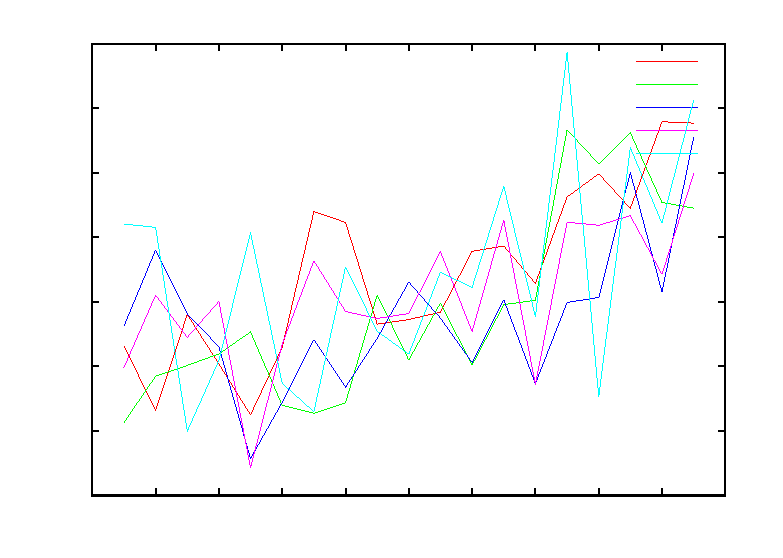
\includegraphics{./plots/randommap80}}%
    \gplfronttext
  \end{picture}%
\endgroup

	\caption{Average path length against map generation probability parameter. 
	15 by 15 map with target in the middle and agents starting on a corner,
	observation probability 0.8, 2500 trials at each point.}
	\label{fig:random80}
\end{figure}
\begin{figure}
	% GNUPLOT: LaTeX picture with Postscript
\begingroup
  \makeatletter
  \providecommand\color[2][]{%
    \GenericError{(gnuplot) \space\space\space\@spaces}{%
      Package color not loaded in conjunction with
      terminal option `colourtext'%
    }{See the gnuplot documentation for explanation.%
    }{Either use 'blacktext' in gnuplot or load the package
      color.sty in LaTeX.}%
    \renewcommand\color[2][]{}%
  }%
  \providecommand\includegraphics[2][]{%
    \GenericError{(gnuplot) \space\space\space\@spaces}{%
      Package graphicx or graphics not loaded%
    }{See the gnuplot documentation for explanation.%
    }{The gnuplot epslatex terminal needs graphicx.sty or graphics.sty.}%
    \renewcommand\includegraphics[2][]{}%
  }%
  \providecommand\rotatebox[2]{#2}%
  \@ifundefined{ifGPcolor}{%
    \newif\ifGPcolor
    \GPcolortrue
  }{}%
  \@ifundefined{ifGPblacktext}{%
    \newif\ifGPblacktext
    \GPblacktexttrue
  }{}%
  % define a \g@addto@macro without @ in the name:
  \let\gplgaddtomacro\g@addto@macro
  % define empty templates for all commands taking text:
  \gdef\gplbacktext{}%
  \gdef\gplfronttext{}%
  \makeatother
  \ifGPblacktext
    % no textcolor at all
    \def\colorrgb#1{}%
    \def\colorgray#1{}%
  \else
    % gray or color?
    \ifGPcolor
      \def\colorrgb#1{\color[rgb]{#1}}%
      \def\colorgray#1{\color[gray]{#1}}%
      \expandafter\def\csname LTw\endcsname{\color{white}}%
      \expandafter\def\csname LTb\endcsname{\color{black}}%
      \expandafter\def\csname LTa\endcsname{\color{black}}%
      \expandafter\def\csname LT0\endcsname{\color[rgb]{1,0,0}}%
      \expandafter\def\csname LT1\endcsname{\color[rgb]{0,1,0}}%
      \expandafter\def\csname LT2\endcsname{\color[rgb]{0,0,1}}%
      \expandafter\def\csname LT3\endcsname{\color[rgb]{1,0,1}}%
      \expandafter\def\csname LT4\endcsname{\color[rgb]{0,1,1}}%
      \expandafter\def\csname LT5\endcsname{\color[rgb]{1,1,0}}%
      \expandafter\def\csname LT6\endcsname{\color[rgb]{0,0,0}}%
      \expandafter\def\csname LT7\endcsname{\color[rgb]{1,0.3,0}}%
      \expandafter\def\csname LT8\endcsname{\color[rgb]{0.5,0.5,0.5}}%
    \else
      % gray
      \def\colorrgb#1{\color{black}}%
      \def\colorgray#1{\color[gray]{#1}}%
      \expandafter\def\csname LTw\endcsname{\color{white}}%
      \expandafter\def\csname LTb\endcsname{\color{black}}%
      \expandafter\def\csname LTa\endcsname{\color{black}}%
      \expandafter\def\csname LT0\endcsname{\color{black}}%
      \expandafter\def\csname LT1\endcsname{\color{black}}%
      \expandafter\def\csname LT2\endcsname{\color{black}}%
      \expandafter\def\csname LT3\endcsname{\color{black}}%
      \expandafter\def\csname LT4\endcsname{\color{black}}%
      \expandafter\def\csname LT5\endcsname{\color{black}}%
      \expandafter\def\csname LT6\endcsname{\color{black}}%
      \expandafter\def\csname LT7\endcsname{\color{black}}%
      \expandafter\def\csname LT8\endcsname{\color{black}}%
    \fi
  \fi
  \setlength{\unitlength}{0.0500bp}%
  \begin{picture}(7200.00,5040.00)%
    \gplgaddtomacro\gplbacktext{%
      \csname LTb\endcsname%
      \put(594,440){\makebox(0,0)[r]{\strut{} 14}}%
      \put(594,982){\makebox(0,0)[r]{\strut{} 16}}%
      \put(594,1524){\makebox(0,0)[r]{\strut{} 18}}%
      \put(594,2066){\makebox(0,0)[r]{\strut{} 20}}%
      \put(594,2608){\makebox(0,0)[r]{\strut{} 22}}%
      \put(594,3149){\makebox(0,0)[r]{\strut{} 24}}%
      \put(594,3691){\makebox(0,0)[r]{\strut{} 26}}%
      \put(594,4233){\makebox(0,0)[r]{\strut{} 28}}%
      \put(594,4775){\makebox(0,0)[r]{\strut{} 30}}%
      \put(726,220){\makebox(0,0){\strut{} 0}}%
      \put(1334,220){\makebox(0,0){\strut{} 0.1}}%
      \put(1941,220){\makebox(0,0){\strut{} 0.2}}%
      \put(2549,220){\makebox(0,0){\strut{} 0.3}}%
      \put(3157,220){\makebox(0,0){\strut{} 0.4}}%
      \put(3765,220){\makebox(0,0){\strut{} 0.5}}%
      \put(4372,220){\makebox(0,0){\strut{} 0.6}}%
      \put(4980,220){\makebox(0,0){\strut{} 0.7}}%
      \put(5588,220){\makebox(0,0){\strut{} 0.8}}%
      \put(6195,220){\makebox(0,0){\strut{} 0.9}}%
      \put(6803,220){\makebox(0,0){\strut{} 1}}%
    }%
    \gplgaddtomacro\gplfronttext{%
      \csname LTb\endcsname%
      \put(5816,4602){\makebox(0,0)[r]{\strut{}Random}}%
      \csname LTb\endcsname%
      \put(5816,4382){\makebox(0,0)[r]{\strut{}Surprise}}%
      \csname LTb\endcsname%
      \put(5816,4162){\makebox(0,0)[r]{\strut{}Entropy}}%
      \csname LTb\endcsname%
      \put(5816,3942){\makebox(0,0)[r]{\strut{}Optimal}}%
      \csname LTb\endcsname%
      \put(5816,3722){\makebox(0,0)[r]{\strut{}Straight Ahead}}%
    }%
    \gplbacktext
    \put(0,0){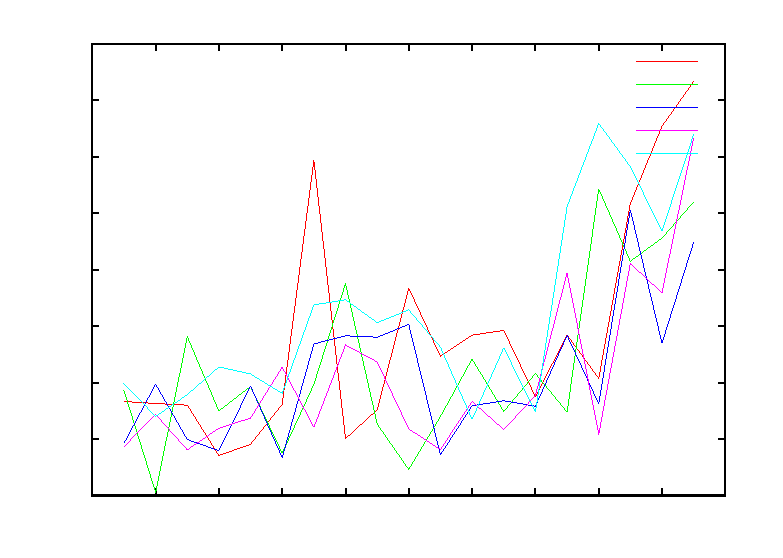
\includegraphics{./plots/randommap90}}%
    \gplfronttext
  \end{picture}%
\endgroup

	\caption{Average path length against map generation probability parameter. 
	15 by 15 map with target in the middle and agents starting on a corner,
	observation probability 0.9, 2500 trials at each point.}
	\label{fig:random90}
\end{figure}

\section{Discussion}
The results of the simulations show no clear winner. This seems remarkable because the 
goal-oriented approach should be behaving optimally at each time step. Given that it is 
often inseparable from a random choice, this does not appear to be the case. In fact this
is not entirely unexpected as the fact that it behaves optimally given its current 
beliefs for a single time step does not mean it is behaving optimally across mutliple.
The current goal-oriented algorithm for sensor choices only considers the impending 
manipulatory action. It is quite probable that were it to look further ahead performance
would increase.

While a simple proposal, this is a difficult problem to solve especially given the 
computational effort required in computing a single step at a time in a complicated
world. A possible avenue is to view the problem as a Partially Observable Markov
Decision Process (POMDP) with the complication that there are two sets of actions with
alternating availability. If this were feasible then there is a significant body of 
techniques for learning policies which would help to approximate truly optimal behaviour
over time. Nevertheless this is still not a simple solution -- POMDPs are very much
an active research area and typical solutions tend to be rather complicated.

Interestingly, in most of the situations tested, the relatively naive approaches of 
trying to minimise entropy of beliefs or maximise information gained from the 
observation performed favourably. On a step-by-step basis these were comparable to the
goal-oriented approach and on the trial that showed some separation between approaches 
both were competitive. This suggests that in the right circumstances (all the maps 
favoured rapid localisation) they might provide a reasonable approximation, despite 
ignoring the possible rewards entirely. Of course this has only been shown in one
particularly contrived scenario, the goal-oriented approach may generalise better to
diverse scenarios and also provides a better framework for extension into multi-step
planning as it is constantly attempting to maximise the expected reward.

The two information-theoretic approaches also differ from the more decision-theoretic
goal-oriented approach in that they are substantially easier to compute (although still
not particularly simple). All are 
polynomial in the number of world states and with the pre-computed table their 
complexity is the same but the goal oriented approach loses as in order to populate the
table it must iterate every pair of sensor actions and observations. This is a 
significant handicap and a good reason to favour one of the less complex approaches.

\section{Conclusion}
While the goal-oriented approach was a narrow winner on an ordered map, particularly 
under greater uncertainty, on a series of randomised maps there was no clear winner.
This is likely due to the lack of ability to plan ahead which hamstrings all of the 
approaches outlined here. The fact that the optimal (in the decision theoretic sense)
performed similarly to some fairly simple, more task specific approaches is encouraging
in that it implies that the full optimal planning process might well able to be shortcut
or estimated in some way.

\printbibliography

\end{document}